\chapter{Moléculas Fotónicas}

La técnica de escritura de guías de onda descrita en el Capítulo~\ref{cap:fs} está restringida por la forma alargada y elíptica del tren de pulsos láser que se enfoca, lo que limita los acoplamientos interorbitales posibles \citep{interorbital}. Una alternativa para aumentar los grados de libertad consiste en fabricar dos guías de onda suficientemente cercanas para hibridizar sus modos guiados, de manera análoga al principio físico que gobierna las moléculas. Por este motivo, en este capítulo se empleará el concepto de \textit{moléculas fotónicas} \citep{molecules}, aplicándolo al estudio experimental de una red fotónica que presenta una doble transición de fase topológica \citep{SPSSH}.

\section{Autoestados del acoplador fotónico para distancias de separación pequeñas}

Como se mencionó en la Sección~\ref{cap:CMT}, la teoría de modos acoplados (CMT) describe adecuadamente los sistemas fotónicos en estudio cuando la distancia entre guías de onda supera los $13\,\mu$m. Para separaciones menores, el sistema debe tratarse como una única macroguía. La expansión en modos normales (EME), presentada en la Sección~\ref{cap:eme}, proporciona una herramienta numérica válida para ambos regímenes. 
Mediante simulaciones de pares de guías de onda a diferentes distancias, se caracterizó el comportamiento de sus autoestados. La Figura~\ref{fig:molecule-coup} muestra que el autoestado antisimétrico ($+-$) solo existe para distancias mayores a $13\,\mu$m, ya que por debajo de este umbral se convierte en un modo de radiación ($k_z^{+-} < k_0 n_0$). En cambio, el autoestado simétrico ($++$) persiste y puede describirse como una única entidad, lo que en esta tesis denominaremos \textit{modo S} de la molécula fotónica.

\begin{figure}[H]
	\centering
	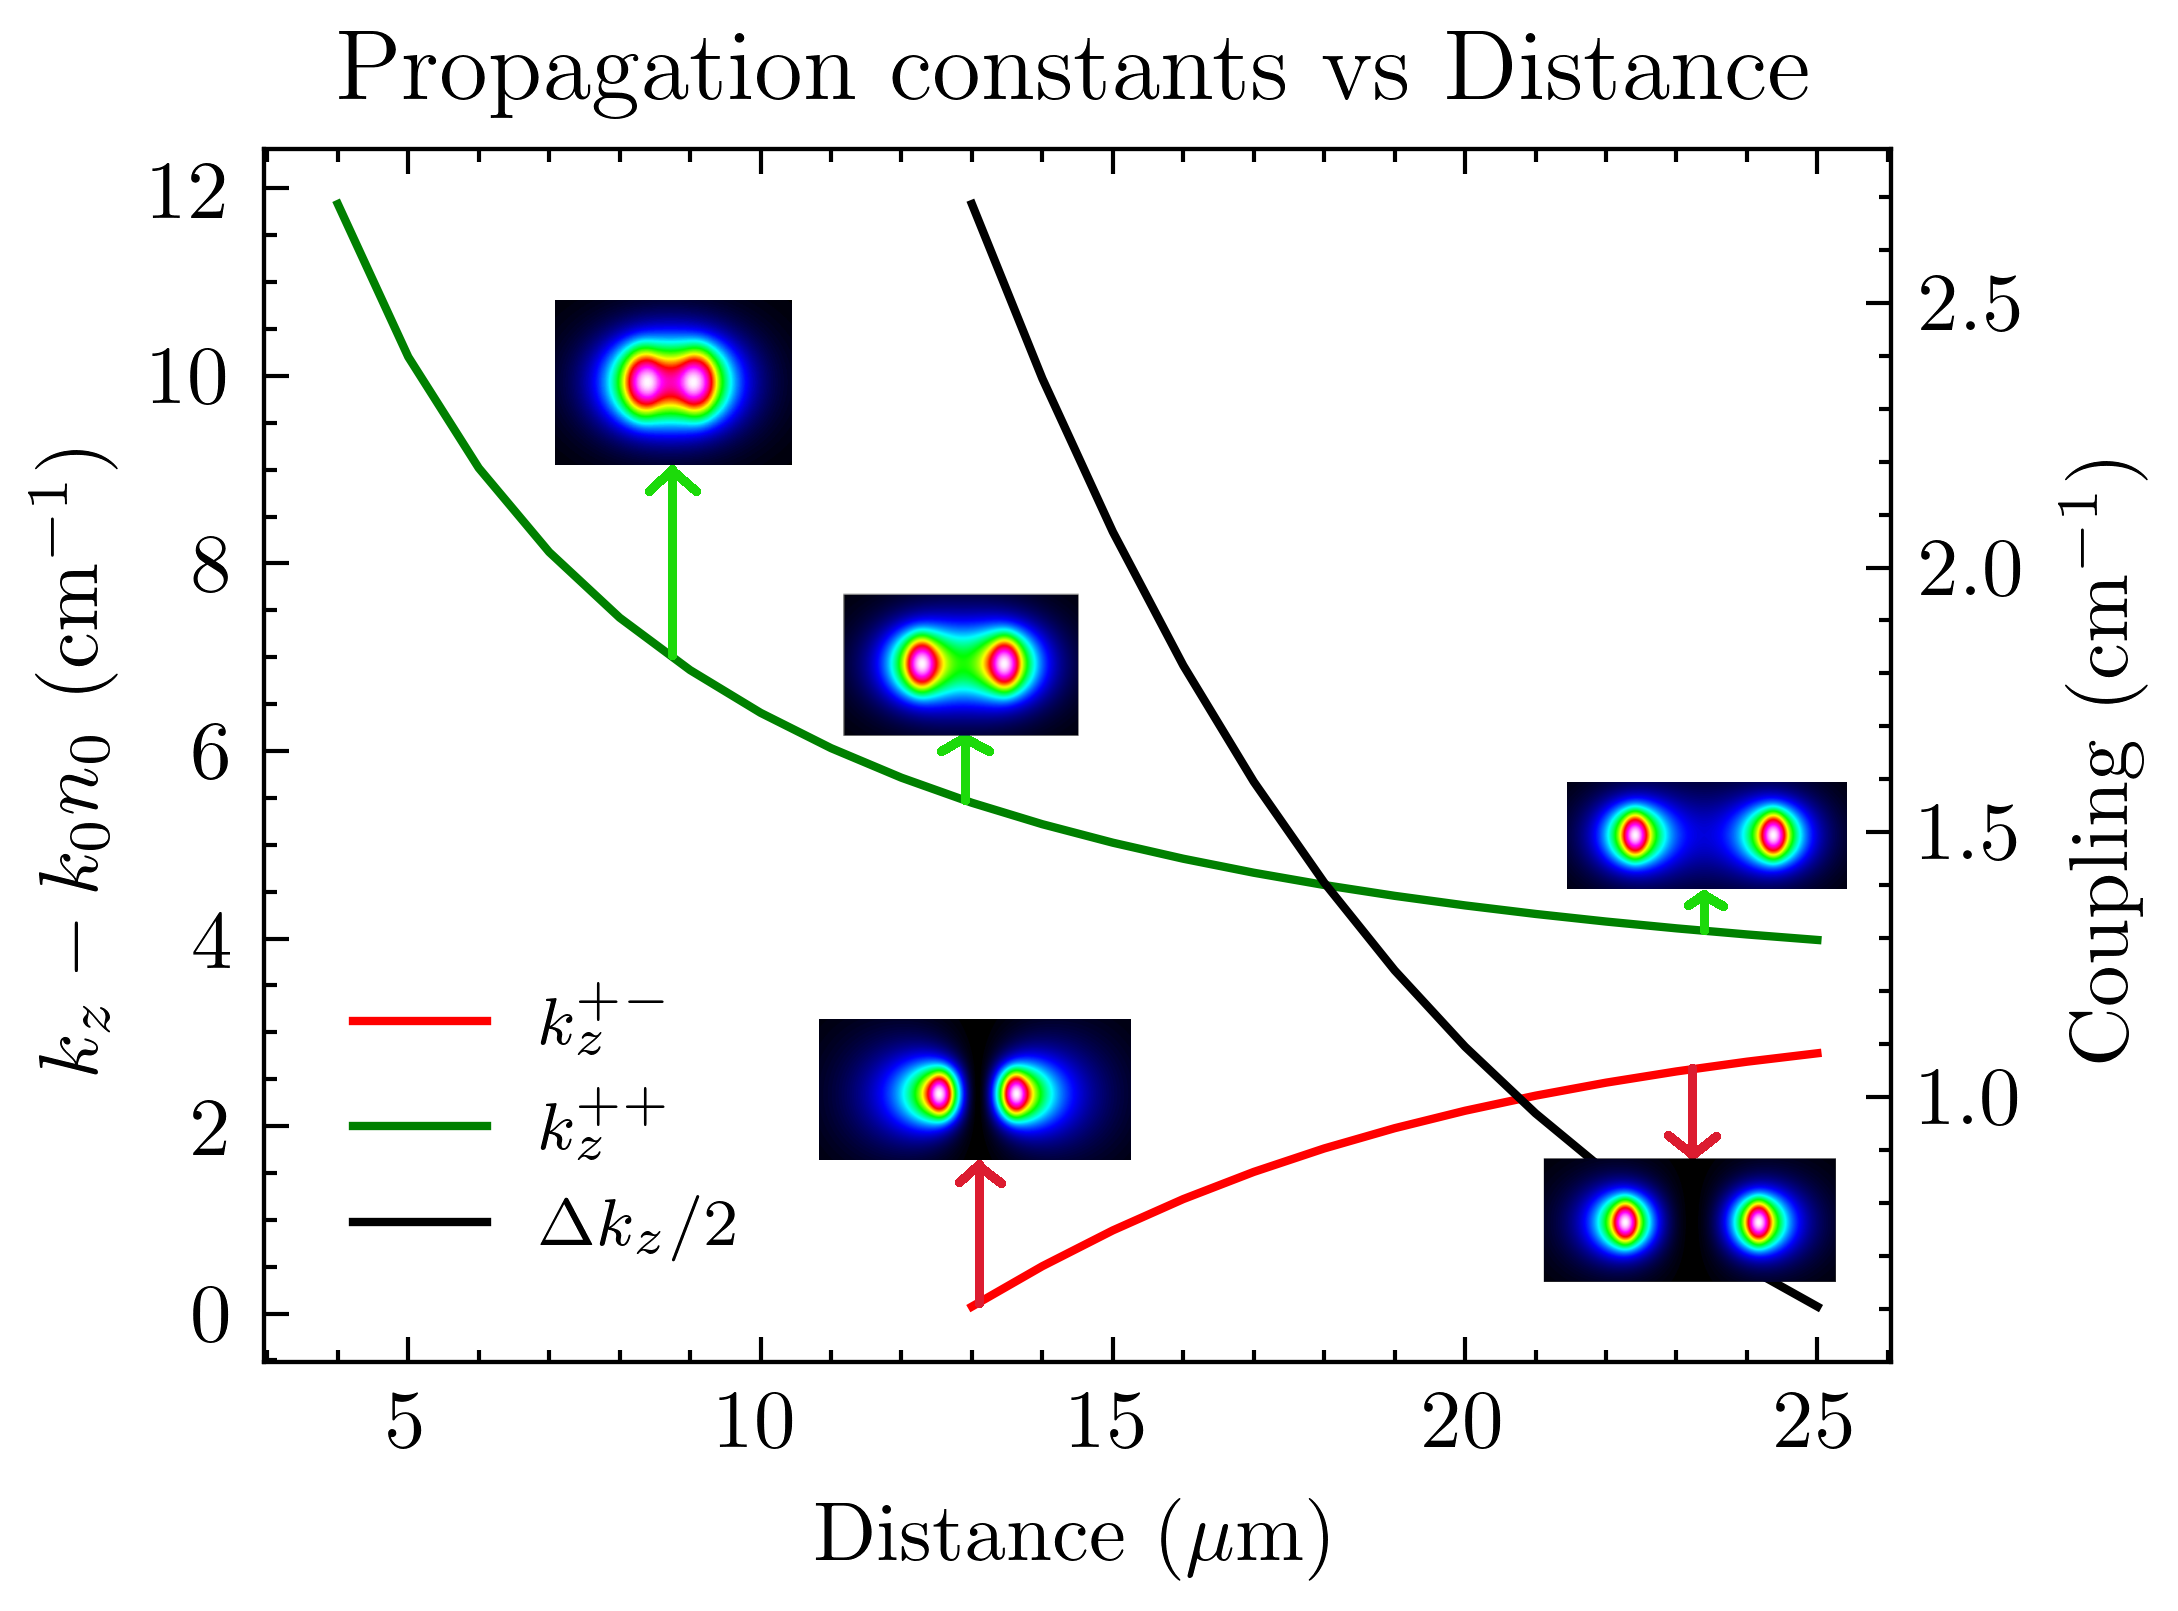
\includegraphics[width=0.50\linewidth]{codigo/dimol2/eigenvalues_vs_angle_1.png}
	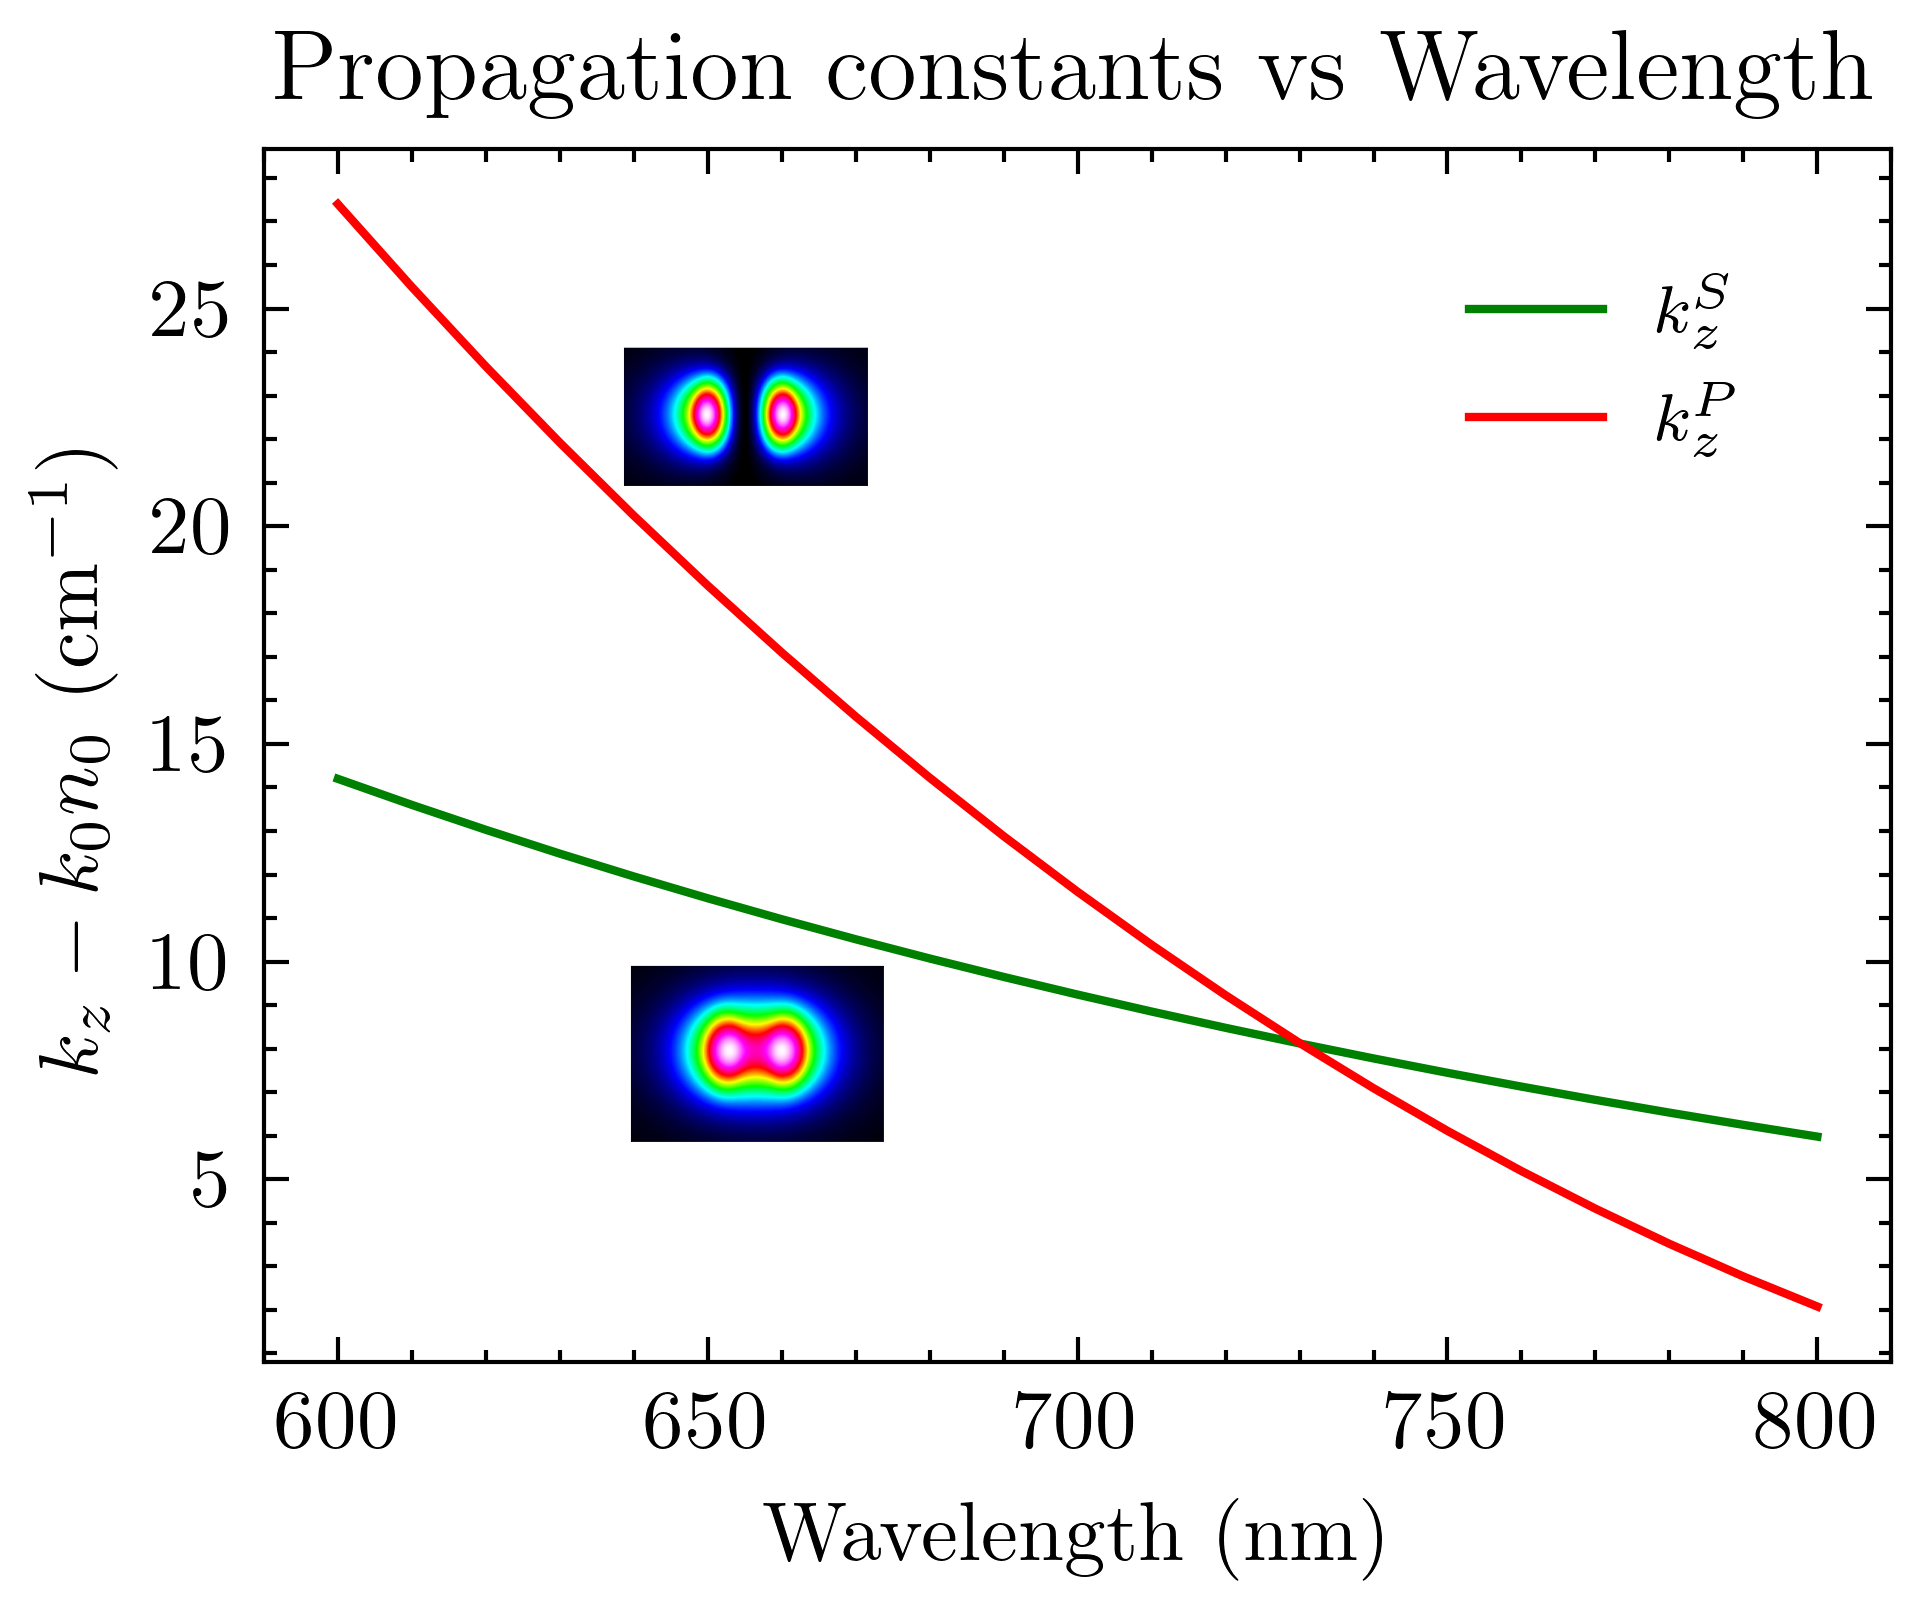
\includegraphics[width=0.45\linewidth]{codigo/dimol3/eigenvalues_vs_wavelength.png}
	\caption[Propagación y acoplamientos en moléculas fotónicas]{
		\textbf{Izquierda:} Constantes de propagación y acoplamientos en función de la distancia para modos fundamentales, calculados mediante EME. 
		\textbf{Derecha:} Constantes de acoplamiento en función de la longitud de onda.
		\label{fig:molecule-coup}}
\end{figure}

Si bien las constantes de propagación de los modos $S$ y $P$ en una misma molécula presentan valores diferentes, estas pueden igualarse entre moléculas adyacentes mediante el ajuste del contraste de índice de refracción en las guías de onda \cite{interorbital}. Por ejemplo, la Figura~\ref{fig:molecule-coup} muestra que a $730$\,nm se igualan las constantes de propagación para $\Delta n_S = 5.200 \times 10^{-4}$ y $\Delta n_P = 10.423 \times 10^{-4}$.


\section{Moléculas Fotónicas en Red SP-SSH}

Para la implementación experimental (sección \ref{cap:fs}) de una red que presente acoplamiento SP \citep{interorbital, SPSSH}, se utilizaron los dipolos horizontales de la sección anterior, obtenidos mediante moléculas fotónicas. Un preciso sintonizado de las constantes de propagación de los modos $s$ y $p$ permitió considerar un grado de libertad análogo al del espín del electrón (\textit{pseudoespín}). El Hamiltoniano $H$ de esta red \citep{SPSSH,toporusos}  es el siguiente

\begin{align*}
	H &= \sum_n \left[\frac{\delta\beta}{2} \left( b^*_{n, 1} b_{n, 1} - a^*_{n, 1} a_{n, 1} + b^*_{n, 2} b_{n, 2} - a^*_{n, 2} a_{n, 2} \right) +k_{ss, 2}a^*_{n, 2} a_{n, 1} -k_{pp, 2}b^*_{n, 2} b_{n, 1} \right. 
	\\	
	&+ k_{ss, 1} \left( a_{n-1, 2}^*a_{n, 1} + a_{n+1, 2}^*a_{n, 2} \right) - k_{pp, 1} \left( b_{n-1, 2}^*b_{n, 1} + b_{n+1, 2}^*b_{n, 2} \right) + k_{sp, 2} \left( a_{n, 2}^* b_{n, 1} - b_{n, 2}^* a_{n, 1} \right)
	\\
	&+ \left. k_{sp, 1} \left( a_{n-1, 2}^* b_{n, 1} - b_{n-1, 2}^* a_{n, 1} + a_{n+1, 1}^*b_{n, 2} - b_{n+1, 1}^* a_{n, 2} \right) \right] + c.c.
\end{align*}

\begin{figure}[H]
\centering
	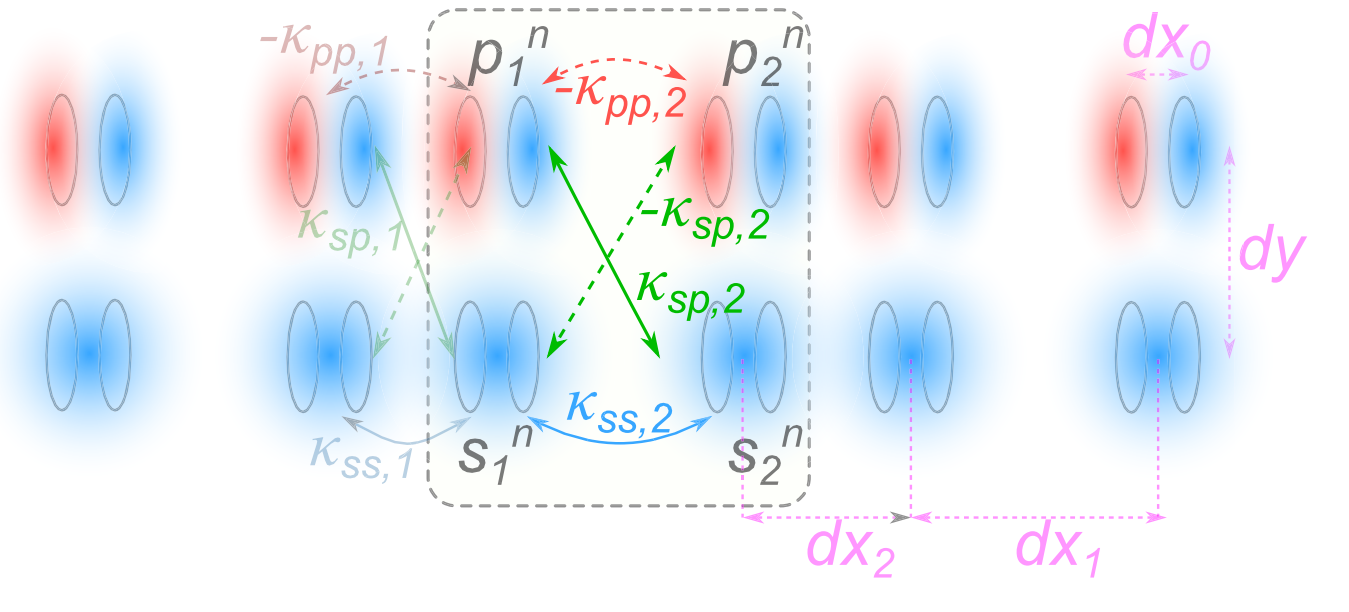
\includegraphics[width=0.7\linewidth]{media/ssh_sp_model}
	\caption{Esquema de la red SP-SSH y los acoplamientos considerados.}
\end{figure}